\documentclass[12pt,a4paper]{article}

% \usepackage[utf8]{inputenc}
% \DeclareUnicodeCharacter{1D12A}{\doublesharp}
% \DeclareUnicodeCharacter{2693}{\anchor}
% \usepackage{dingbat}
% \DeclareRobustCommand\dash\unskip\nobreak\thinspace{\textemdash\allowbreak\thinspace\ignorespaces}
\usepackage[top=2in, bottom=1in, left=1in, right=1in]{geometry}
%\usepackage{fullpage}

\usepackage{tabularx}
\usepackage{multirow}
\usepackage{makecell}
\usepackage{fancyhdr}\pagestyle{fancy}\rhead{University of California -- Los Angeles Spring 2020}\lhead{Math 156 Term Project 1}

\usepackage{enumitem}

\usepackage{amsmath,amssymb,amsthm,amsfonts,microtype,stmaryrd}
	%{mathtools,wasysym,yhmath}

\usepackage[usenames,dvipsnames]{xcolor}
\newcommand{\blue}[1]{\textcolor{blue}{#1}}
\newcommand{\red}[1]{\textcolor{red}{#1}}
\newcommand{\gray}[1]{\textcolor{gray}{#1}}
\newcommand{\fgreen}[1]{\textcolor{ForestGreen}{#1}}

\usepackage{mdframed}
	%\newtheorem{mdexample}{Example}
	\definecolor{warmgreen}{rgb}{0.8,0.9,0.85}
	% --Example:
	% \begin{center}
	% \begin{minipage}{0.7\textwidth}
	% \begin{mdframed}[backgroundcolor=warmgreen, 
	% skipabove=4pt,skipbelow=4pt,hidealllines=true, 
	% topline=false,leftline=false,middlelinewidth=10pt, 
	% roundcorner=10pt] 
	%%%% --CONTENTS-- %%%%
	% \end{mdframed}\end{minipage}\end{center}	

\usepackage{graphicx} \graphicspath{{}}
	% --Example:
	% \includegraphics[scale=0.5]{picture name}
%\usepackage{caption} %%% --some awful package to make caption...

\usepackage{hyperref}\hypersetup{linktocpage,colorlinks}\hypersetup{citecolor=black,filecolor=black,linkcolor=black,urlcolor=blue,breaklinks=true}

%%% --Text Fonts
%\usepackage{times} %%% --Times New Roman for LaTeX
%\usepackage{fontspec}\setmainfont{Times New Roman} %%% --Times New Roman; XeLaTeX only

%%% --Math Fonts
\renewcommand{\v}[1]{\ifmmode\mathbf{#1}\fi}
%\renewcommand{\mbf}[1]{\mathbf{#1}} %%% --vector
%\newcommand{\ca}[1]{\mathcal{#1}} %%% --"bigO"
%\newcommand{\bb}[1]{\mathbb{#1}} %%% --"Natural, Real numbers"
%\newcommand{\rom}[1]{\romannumeral{#1}} %%% --Roman numbers

%%% --Quick Arrows
\newcommand{\ra}[1]{\ifnum #1=1\rightarrow\fi\ifnum #1=2\Rightarrow\fi\ifnum #1=3\Rrightarrow\fi\ifnum #1=4\rightrightarrows\fi\ifnum #1=5\rightleftarrows\fi\ifnum #1=6\mapsto\fi\ifnum #1=7\iffalse\fi\fi\ifnum #1=8\twoheadrightarrow\fi\ifnum #1=9\rightharpoonup\fi\ifnum #1=0\rightharpoondown\fi}

%\newcommand{\la}[1]{\ifnum #1=1\leftarrow\fi\ifnum #1=2\Leftarrow\fi\ifnum #1=3\Lleftarrow\fi\ifnum #1=4\leftleftarrows\fi\ifnum #1=5\rightleftarrows\fi\ifnum #1=6\mapsfrom\ifnum #1=7\iffalse\fi\fi\ifnum #1=8\twoheadleftarrow\fi\ifnum #1=9\leftharpoonup\fi\ifnum #1=0\leftharpoondown\fi}

%\newcommand{\ua}[1]{\ifnum #1=1\uparrow\fi\ifnum #1=2\Uparrow\fi}
%\newcommand{\da}[1]{\ifnum #1=1\downarrow\fi\ifnum #1=2\Downarrow\fi}

%%% --Special Editor Config
\renewcommand{\ni}{\noindent}
\newcommand{\onum}[1]{\raisebox{.5pt}{\textcircled{\raisebox{-1pt} {#1}}}}

\newcommand{\claim}[1]{\underline{``{#1}":}}

\renewcommand{\l}{\left}\renewcommand{\r}{\right}

\newcommand{\casebrak}[4]{\left \{ \begin{array}{ll} {#1},&{#2}\\{#3},&{#4} \end{array} \right.}
%\newcommand{\ttm}[4]{\l[\begin{array}{cc}{#1}&{#2}\\{#3}&{#4}\end{array}\r]} %two-by-two-matrix
%\newcommand{\tv}[2]{\l[\begin{array}{c}{#1}\\{#2}\end{array}\r]}

\def\dps{\displaystyle}

\let\italiccorrection=\/
\def\/{\ifmmode\expandafter\frac\else\italiccorrection\fi}


%%% --General Math Symbols
\def\bc{\because}
\def\tf{\therefore}

%%% --Frequently used OPERATORS shorthand
\newcommand{\INT}[2]{\int_{#1}^{#2}}
% \newcommand{\UPINT}{\bar\int}
% \newcommand{\UPINTRd}{\overline{\int_{\bb R ^d}}}
\newcommand{\SUM}[2]{\sum\limits_{#1}^{#2}}
\newcommand{\PROD}[2]{\prod\limits_{#1}^{#2}}
\newcommand{\CUP}[2]{\bigcup\limits_{#1}^{#2}}
\newcommand{\CAP}[2]{\bigcap\limits_{#1}^{#2}}
% \newcommand{\SUP}[1]{\sup\limits_{#1}}
% \newcommand{\INF}[1]{\inf\limits_{#1}}
\DeclareMathOperator*{\argmin}{arg\,min}
\DeclareMathOperator*{\argmax}{arg\,max}
\newcommand{\pd}[2]{\frac{\partial{#1}}{\partial{#2}}}
\def\tr{\text{tr}}

\renewcommand{\o}{\circ}
\newcommand{\x}{\times}
\newcommand{\ox}{\otimes}

\newcommand\ie{{\it i.e. }}
\newcommand\wrt{{w.r.t. }}
\newcommand\dom{\mathbf{dom\:}}

%%% --Frequently used VARIABLES shorthand
\newcommand{\R}{\ifmmode\mathbb R\fi}
\newcommand{\N}{\ifmmode\mathbb N\fi}
\renewcommand{\O}{\mathcal{O}}
\newcommand{\w}{\wedge}
\newcommand{\ome}{\omega}
\newcommand{\lam}{\lambda}
\newcommand{\im}{\mbox{im}}

\newcommand{\B}{\mathcal B}
\newcommand{\var}{\mbox{var}}
\newcommand{\E}{\mathbb{E}}

%\usepackage{showkeys}
%%%%%%%%%%%%%%%%%%%%%%%%%%%%%%%%%%%%%%%%%%%%%%%%%%%%%%%%%%%%%%%%%%%%%%%%%%%%%%%%%%%%%%%%%%%%%%%%%%%%%%%%%%%%%%%%%%%%%%%%%%%%%%%%%%%%%%%%%%%%%%%%%%%%%%%%%%%%%%%%%%%%%%%%%%%%%%%%%%%%%%%%%%%%%%%%%%%%%%
\begin{document}
\title{Math 156 Term Project 1}
\author{\textbf{Deadline:} Saturday April 18th 11:59pm}
\date{}
\maketitle

\subsubsection*{Problem 1}
Explain in your own words the benefit of maximizing the log likelihood compared to directly maximizing the likelihood function. You will have to write a few complete (English) sentences along with some supplementary mathematical formulas to answer this question. (20 points)

\subsubsection*{Problem 2}
(a) Give an example of continuous data, i.e. a data set for which we can use a continuous random variable to model. (5 points) \\
(b) Give an example of discrete data, i.e. a data set for which we need to use a discrete random variable. (5 points) \\
(c) Prove that $\var[f] = \mathbb E[f(x)^2] - \mathbb E[f(x)]^2$ for both continuous and discrete random variables. Recall the definition of variance of $f(x)$ is defined by
\begin{equation*}
\var[f] = \E[ (f(x) - \E[f(x)])^2 ].
\end{equation*}
(Feel free to use measure theory to give a unifying proof for both.) (10 points)


\subsubsection*{Problem 3}
Suppose we have a data set $\mathcal D = (\v x, \v t), \v x= (x_1, \cdots, x_N), \v t = (t_1, \cdots, t_N)$ generated by
\begin{equation*}
t_i = f(x_i) + \mbox{noise},
\end{equation*}
where $f: \R \ra1 \R$ is an unknown function of interest. $N$ is the number of data points given. We can assume the noise is some Gaussian noise with mean zero, i.e. each noise is independent of each other and $\sim \mathcal N(0, \beta^{-1})$ for some unknown parameter $\beta>0$. Figure~\ref{fig:N20} shows the data provided with $N=20$.
%
\begin{figure}[h]
\centering
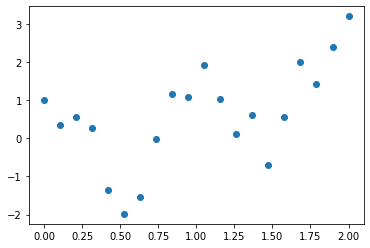
\includegraphics[scale=0.6]{TP1_fitting_N20}
\caption{Scatter plot of \texttt{fitting\_N20.csv}.}
\label{fig:N20}
\end{figure}
%
We would like to use this data set to approximate $f$ using a function of the form
%
\begin{equation*} 
y(x,\v{w})=w_0+w_1x+w_2x^2+\cdots+w_Mx^M=\sum_{j=0}^M w_j x^j, 
\end{equation*}
%
where $M \geq 2$ (degree of the polynomial) and $\v w = (w_0, w_1, \cdots, w_M) \in \R^{M+1}$ (polynomial coefficients) are parameters to be determined by you. Use everything we taught in class (and reference to textbook \S1.1 and \S1.2.5) to finish the following tasks. 
%
\begin{enumerate}[label=(\alph*)]
\item Formulate the problem into a minimization or maximization problem. What is your cost function? (Feel free to add regularizer if you deem suitable.) Your answer to this question should be handwritten math equations or typed in \LaTeX. (Hint: they are provided on textbook p.5, p.29, or p.30.) (10 points)
\item Read the data into your program from the csv file \texttt{fitting\_N20.csv} and create a plot similar to Figure~\ref{fig:N20}. (5 points)
\item Solve the problem numerically, that is, write a program that takes the data in \texttt{fitting\_N20.csv} and compute the corresponding optimal coefficients $\v w^\ast = (w_0^\ast, w_1^\ast, w_2^\ast, \cdots, w_M^\ast)$. Write down your plan for solving this problem in math equations or pseudocode (or type in \LaTeX) for partial credit. (25 points) 
\item Plot your fitting function $y(x, \v w)$ as a curve alongside the data. The following graph in Figure~\ref{fig:curve} is an example for you. (10 points) 
\begin{figure}[h]
\centering
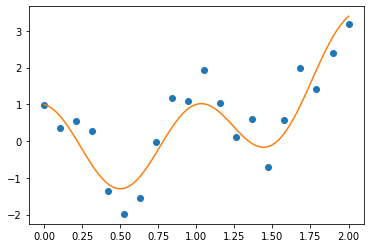
\includegraphics[scale=0.6]{TP1_fitting_N20_curve} 
\caption{Sample plot for task (d).}
\label{fig:curve}
\end{figure}
\item What is your choice of $M$? Why? You can performed the above tasks with a few different choices of $M$, or give a convincing heuristic argument. (20 points)
\item \textbf{(Bonus)} You can find \texttt{fitting\_N50.csv} on the course website. It is generated with the same process as \texttt{fitting\_N20.csv}, except with more data point in the same interval $[0, 2]$. See Figure~\ref{fig:N50}. Note that this data set is obtained with the same kind of random noise ($\sim \mathcal N(0, \beta^{-1})$). Use this however you wish to generate more information and explain how a larger data set helps with your work. (up to 20 points)
\begin{figure}[h]
\centering
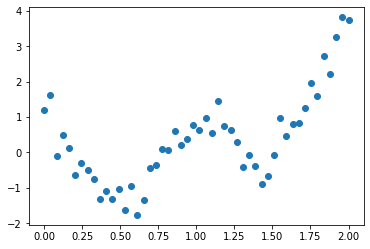
\includegraphics[scale=0.6]{TP1_fitting_N50}
\caption{Scatter plot for \texttt{fitting\_N50.csv}.}
\label{fig:N50}
\end{figure}
\end{enumerate}
%
\textbf{Important submission note:}
You can use any programming language to accomplish the coding tasks. The university now provides MATLAB access to all UCLA students, see \href{https://www.it.ucla.edu/news/matlab-software-now-available}{https://www.it.ucla.edu/news/matlab-software-now-available}. Other high-level programming languages suitable for our tasks include Python, R, Julia, Octave, and more. The instructor and the TA guarantee assistance with MATLAB programming and can potentially help you trouble shoot your code in other programming languages (not guaranteed). If you wish to email us asking for programming assistance, please attach your code, highlight the part in question, and articulate your problems. Please attach your code at the end of your submission and document a list of your collaborators and external resource. This document is created with \LaTeX{} and you can find the source .tex file on CCLE. For more \LaTeX{} help, check out \href{https://www.maths.tcd.ie/~dwilkins/LaTeXPrimer/}{this \LaTeX{} tutorial link}, or take a look at my \href{https://raw.githubusercontent.com/evastgh/ps/master/template.tex}{template .tex file}. \\
\\
The following table is the data provided in \texttt{fitting\_N20.csv} for your visual inspection. 
\begin{center}
\resizebox{0.3\textwidth}{!}{
\begin{tabular}{|c|c|c|}
\hline
  $i$ & $x_i$ & $t_i$ \\
  \hline
1 &   0.000000 &   0.991459 \\
2 &   0.105263 &   0.360328 \\
3 &   0.210526 &   0.558448 \\
4 &   0.315789 &   0.265560 \\
5 &   0.421053 &  -1.364200 \\
6 &   0.526316 &  -1.983883 \\
7 &   0.631579 &  -1.551820 \\
8 &   0.736842 &  -0.020161 \\
9 &   0.842105 &   1.164831 \\
10 &   0.947368 &   1.090539 \\
11 &   1.052632 &   1.925967 \\
12 &   1.157895 &   1.031809 \\
13 &   1.263158 &   0.099923 \\
14 &   1.368421 &   0.608555 \\
15 &   1.473684 &  -0.701440 \\
16 &   1.578947 &   0.566558 \\
17 &   1.684211 &   1.998774 \\
18 &   1.789474 &   1.423031 \\
19 &   1.894737 &   2.386509 \\
20 &   2.000000 &   3.199598 \\
\hline
\end{tabular}
}
\end{center}





\end{document}



